% SPDX-License-Identifier: MIT-0
\documentclass[11pt,a4paper]{article}
\usepackage[T1]{fontenc}
\usepackage[utf8]{inputenc}
\usepackage{lmodern}
\usepackage[margin=25mm,headheight=14pt]{geometry}
\usepackage{amsmath,amssymb,amsthm,mathtools}
\usepackage{microtype,booktabs,longtable,array,graphicx,multicol}
\usepackage{enumitem,fancyhdr}
\usepackage[numbers,sort&compress]{natbib}
\usepackage[hidelinks]{hyperref}
\usepackage{listings}
\hypersetup{pdftitle={Exact eventual maximizers of Rudin--Shapiro autocorrelations},
 pdfauthor={AI-assisted research draft prepared for Vladimir Reshetnikov},
 pdfsubject={A rational polytope certificate for the uniqueness and location conjecture}}
\pagestyle{fancy}\fancyhf{}
\fancyhead[L]{\small Rudin--Shapiro autocorrelation maxima}
\fancyhead[R]{\small Research draft}
\fancyfoot[C]{\thepage}
\setlength{\parskip}{0.25em}
\setlength{\emergencystretch}{2em}
\setcounter{tocdepth}{2}
\newtheorem{theorem}{Theorem}[section]
\newtheorem{lemma}[theorem]{Lemma}
\newtheorem{proposition}[theorem]{Proposition}
\newtheorem{corollary}[theorem]{Corollary}
\theoremstyle{definition}\newtheorem{definition}[theorem]{Definition}
\theoremstyle{remark}\newtheorem{remark}[theorem]{Remark}
\newcommand{\R}{\mathbb R}
\newcommand{\Q}{\mathbb Q}
\newcommand{\Z}{\mathbb Z}
\newcommand{\conv}{\operatorname{conv}}
\newcommand{\diag}{\operatorname{diag}}
\newcommand{\sgn}{\operatorname{sgn}}
\newcommand{\tr}{\mathsf T}
\newcommand{\ee}{\varepsilon}
\newcommand{\cB}{\mathcal B}
\newcommand{\cR}{\mathcal R}
\newcommand{\cP}{\mathcal P}
\newcommand{\cK}{\mathcal K}
\newcommand{\vv}{\begin{pmatrix}1\\-1\\1\end{pmatrix}}
\newcommand{\state}[3]{\begin{pmatrix}#1\\#2\\#3\end{pmatrix}}
\lstset{basicstyle=\ttfamily\small,breaklines=true,columns=fullflexible,
 keepspaces=true,showstringspaces=false,frame=single,framerule=0.3pt}

\title{\textbf{Exact eventual maximizers of\newline Rudin--Shapiro autocorrelations}\\[0.55em]
\large A rational polytope certificate for the uniqueness-and-location conjecture}
\author{AI-assisted research draft\\\small Prepared for Vladimir Reshetnikov}
\date{20 September 2026}

\begin{document}
\maketitle
\begin{abstract}
For the Rudin--Shapiro sequence of length $2^m$, let $C_m(k)$ denote its
aperiodic autocorrelation and let $A_m=\max_{0<k<2^m}|C_m(k)|$.
We give a proposed computer-assisted proof that the maximizing positive shift
is unique for every $m\ge3$ and, more strongly, that
\[
 k_m^*=\frac{2^{m+1}+(-1)^m}{3}\qquad(m\ge40).
\]
The threshold $40$ is sharp. Thus the location conjecture of Tarnu, reiterated
as Conjecture~1.5 of Choi--Tarnu, follows after recording the elementary
exception at $m=2$; Tarnu's further question about infinitely many
nearest-integer maximizers receives an eventual-equality answer.
The proof reduces all autocorrelations to words in two integer matrices.
A finite calculation is certified by convex combinations, and a moving
26-point polytope supplies the induction for every subsequent level.
Its containment conditions are polynomial inequalities over a rational
rectangle. A six-step projective trapping argument uses rational arithmetic
only. We also obtain an exact eventual cubic recurrence, the limiting
constant for $A_m/\lambda^m$, a rational generating function for $A_m$, and
an eventual classification of periodic maximizers.
The accompanying standard-library Python verifier has been run successfully;
it does not trust numerical convex-hull or eigenvalue calculations.
\end{abstract}

\begin{center}
\begin{minipage}{0.92\textwidth}\small
\textbf{Status.} This is an unrefereed proposed proof with executed exact
arithmetic certificates, not an independently reviewed result or a
proof-assistant formalization. The mathematical reduction, the certificate
format, and the boundary between discovery and verification are explicit below.
\end{minipage}
\end{center}
\clearpage
\tableofcontents
\clearpage

\section{The problem and the result}
\label{sec:result}

For $j\ge0$, put
\[
 r_j=(-1)^{\text{number of overlapping occurrences of $11$ in the binary expansion of $j$}}.
\]
The level-$m$ Rudin--Shapiro sequence is $(r_0,\ldots,r_{2^m-1})$.
Its positive-shift aperiodic autocorrelations and peak sidelobe level are
\begin{equation}
 C_m(k)=\sum_{j=0}^{2^m-1-k}r_jr_{j+k},\qquad
 A_m=\max_{1\le k<2^m}|C_m(k)|.
 \label{eq:definition}
\end{equation}
The main lobe $C_m(0)=2^m$ is not included in this maximum.
Negative shifts introduce only the symmetry $C_m(-k)=C_m(k)$, so uniqueness
always means uniqueness among positive shifts.

Tarnu's concluding conjecture asks for uniqueness and
$k_m^*/2^m\to2/3$; the same section asks whether the nearest integer to
$2^{m+1}/3$ maximizes infinitely often \citep[Section~4]{Tarnu2023}.
Choi and Tarnu retain the discrete conjecture as Conjecture~1.5 in their 2025
paper and study a related limit model on the unit interval
\citep[Conjecture~1.5 and Section~4]{ChoiTarnu2025}.
We attack the discrete question directly.

There is one necessary small-index convention. At $m=2$,
\[
 (C_2(1),C_2(2),C_2(3))=(1,0,-1),
\]
so both $1$ and $3$ maximize the absolute value. The literal phrase
``for each $m$'' needs this exception. The substantive assertion studied here
is uniqueness for $m\ge3$, not a disproof based on that elementary tie.

Define
\begin{equation}
 \ell_m=\frac{2^{m+1}+(-1)^m}{3}.
 \label{eq:ell}
\end{equation}
This is an odd integer and is the nearest integer to $2^{m+1}/3$.
Let the integer sequence $(b_n)_{n\ge0}$ be defined by
\begin{equation}
 b_0=1,\quad b_1=1,\quad b_2=5,\qquad
 b_n=-b_{n-1}+2b_{n-2}+4b_{n-3}\quad(n\ge3).
 \label{eq:b-recurrence}
\end{equation}

\begin{theorem}[Exact eventual maximizers]
\label{thm:main}
For every integer $m\ge3$, the maximum in \eqref{eq:definition} is attained
at exactly one positive shift $k_m^*$. For every $m\ge40$,
\begin{equation}
 k_m^*=\ell_m,\qquad
 C_m(k_m^*)=(-1)^{m-1}b_{m-2},\qquad A_m=b_{m-2}.
 \label{eq:main}
\end{equation}
The threshold $40$ cannot be reduced. For $3\le m<40$, all departures from
$k_m^*=\ell_m$ are exactly those in Table~\ref{tab:exceptions}.
The table also gives every nonzero correction $A_m-b_{m-2}$.
\end{theorem}

\begin{table}[htbp]
\centering
\caption{The complete exceptional set. At every unlisted $m\ge3$, both
$k_m^*-\ell_m$ and $A_m-b_{m-2}$ are zero.}
\label{tab:exceptions}
\begin{tabular}{rrr}
\toprule
$m$ & $k_m^*-\ell_m$ & $A_m-b_{m-2}$\\
\midrule
3 & $-2$ & $2$ \\
5 & $-8$ & $6$ \\
7 & $-34$ & $10$ \\
8 & $2$ & $12$ \\
9 & $22$ & $4$ \\
10 & $8$ & $56$ \\
12 & $34$ & $116$ \\
13 & $86$ & $52$ \\
14 & $136$ & $64$ \\
15 & $-8$ & $408$ \\
17 & $1{,}110$ & $1{,}084$ \\
19 & $4{,}352$ & $952$ \\
20 & $2$ & $2{,}444$ \\
22 & $8$ & $8{,}696$ \\
24 & $34$ & $10{,}868$ \\
25 & $-2$ & $6{,}492$ \\
27 & $-8$ & $63{,}000$ \\
29 & $-34$ & $84{,}644$ \\
32 & $2$ & $325{,}580$ \\
34 & $8$ & $616{,}568$ \\
39 & $-2$ & $1{,}897{,}468$ \\
\bottomrule
\end{tabular}
\end{table}

For example, the last exception is
\begin{align*}
 \ell_{39}&=366503875925, & k_{39}^*&=366503875923,\\
 C_{39}(\ell_{39})&=132094089, & A_{39}&=133991557.
\end{align*}
At the next three levels,
\begin{equation}
 (A_{40},A_{41},A_{42})=(255886741,372089521,668060317).
 \label{eq:initial-eventual}
\end{equation}
The exceptional data are recomputed from the defining sequences and matrix
recurrences, rather than transcribed from a published numerical table.

\begin{figure}[htbp]
\centering
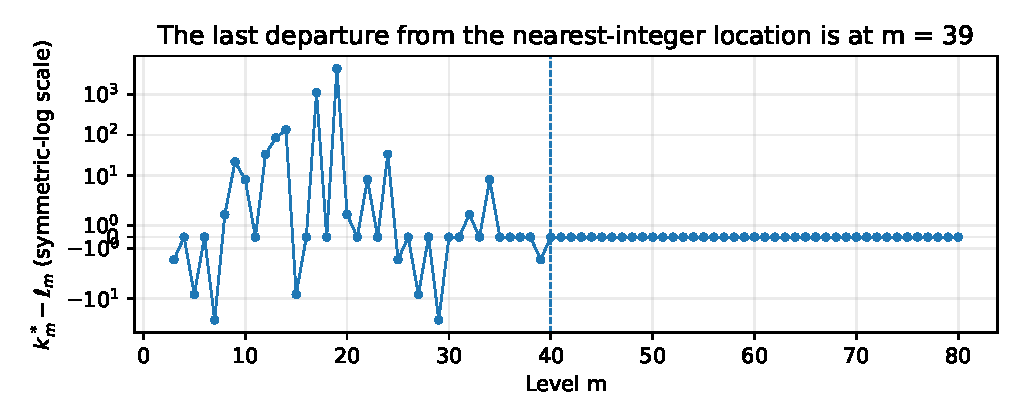
\includegraphics[width=\textwidth]{figures/maximizer_deviation.pdf}
\caption{Exact maximizing-shift deviations, displayed on a symmetric-log
vertical scale to show both the large early departures and the final departure
of $-2$. The plotted finite data are certified; the all-level statement comes
from the induction in Sections~\ref{sec:polytope}--\ref{sec:assembly}.}
\end{figure}

\subsection{What is new here, and what is not}
The exponential scale $A_m\asymp\lambda^m$, where
$\lambda=1.658967\ldots$ solves $\lambda^3+\lambda^2-2\lambda-4=0$, is
established work. In particular, Katz and van der Linden prove the sharp
uniform prefactor bound $A_m\le5\lambda^{m-4}$
\citep{KatzLinden2022}. The autocorrelation recurrences and the use of
matrix products are also prior work; we rederive the recurrences to make the
argument self-contained. Tarnu already discusses numerical invariant
polytopes for the associated joint spectral radius
\citep[Section~3]{Tarnu2023}.

The claimed contribution is the exact all-level maximizing shift, its
uniqueness, and the sharp onset $40$, together with certificates establishing
these assertions. A growth-rate bound does not specify which word in the
matrices maximizes a particular coordinate. Likewise, a pointwise limit model
with a unique maximum does not by itself control the maximizers of the finite
functions. Our moving polytope is tied to the particular reference orbit
$U^n v$ and controls those finite coordinate extrema.

\section{A self-contained autocorrelation recurrence}
\label{sec:recurrence}

Let $p_0(z)=q_0(z)=1$, and recursively define
\begin{equation}
 p_m(z)=p_{m-1}(z)+z^{2^{m-1}}q_{m-1}(z),\qquad
 q_m(z)=p_{m-1}(z)-z^{2^{m-1}}q_{m-1}(z).
 \label{eq:rs-polynomials}
\end{equation}
The coefficients of $p_m$ are $r_0,\ldots,r_{2^m-1}$. Indeed, appending a
leading binary $1$ creates exactly one additional $11$ when the next binary
digit is $1$; and the coefficients of $q_m$ agree with those of $p_m$ in its
first half and have the opposite signs in its second half.

For a real-coefficient Laurent polynomial, write $f^*(z)=f(z^{-1})$.
On the unit circle, $f(z)f^*(z)=|f(z)|^2$. Directly from
\eqref{eq:rs-polynomials},
\begin{equation}
 p_m p_m^*+q_m q_m^*=2^{m+1}.
 \label{eq:complementarity}
\end{equation}
Consequently the nonconstant coefficients of the two squared moduli cancel.
This is also the Fourier-analytic interpretation of the problem:
\begin{equation}
 |p_m(e^{i\theta})|^2
 =2^m+2\sum_{k=1}^{2^m-1}C_m(k)\cos(k\theta).
 \label{eq:fourier}
\end{equation}
We seek the largest nonconstant Fourier coefficient in absolute value.

Put $H_n(z)=q_n(z)p_n^*(z)$ and $h_n(t)=[z^t]H_n(z)$.
If $L=2^{m-1}$, expanding $p_mp_m^*$ and using
\eqref{eq:complementarity} gives
\[
 p_mp_m^*=2^m+z^L H_{m-1}+z^{-L}H_{m-1}^*.
\]
The first cross term has only positive powers, and the second only negative
powers. Thus, for $0<k<2^m$,
\begin{equation}
 C_m(k)=h_{m-1}(k-L).
 \label{eq:mixed}
\end{equation}
Similarly, with $h=2^{n-1}$,
\[
 H_n=2p_{n-1}p_{n-1}^*-2^n+z^{-h}H_{n-1}^*-z^hH_{n-1}.
\]
Its constant coefficient is zero for $n\ge1$. For $t\ne0$, its other
coefficients satisfy
\begin{equation}
 h_n(t)=2C_{n-1}(|t|)-\sgn(t)C_n(|t|),
 \label{eq:h-coeff}
\end{equation}
where a correlation outside its support is zero.
Equations~\eqref{eq:mixed} and \eqref{eq:h-coeff} prove the following recurrence.

\begin{lemma}
\label{lem:scalar}
For $m\ge3$, $C_m(2^{m-1})=0$. For $0<k<2^m$ and $k\ne2^{m-1}$,
\begin{equation}
 C_m(k)=
 \begin{cases}
 C_{m-1}(2^{m-1}-k)+2C_{m-2}(2^{m-1}-k), & k<2^{m-1},\\
 -C_{m-1}(k-2^{m-1})+2C_{m-2}(k-2^{m-1}), & k>2^{m-1}.
 \end{cases}
 \label{eq:scalar}
\end{equation}
Every nonzero even shift has $C_m(k)=0$ for $m\ge2$.
\end{lemma}

\begin{proof}
Only the last assertion remains. It holds at $m=2$. At a noncentral even
shift, the arguments on the right of \eqref{eq:scalar} are positive and even,
so induction applies; at the central shift, use $h_{m-1}(0)=0$.
\end{proof}

When $k$ is in the first or fourth quarter of the full shift interval, the
$C_{m-2}$ term vanishes by its support. Thus \eqref{eq:scalar} also yields
the familiar four-quarter version of the recurrence. The proof above uses
only finite Laurent-polynomial identities, without convergence or asymptotic
interchanges.

\section{Two matrices and a bijective address system}
\label{sec:matrices}

For an odd $k$ with $0<k<2^{m-1}$, define the lower-half state
\begin{equation}
 w_m(k)=\state{C_m(k)}{C_m(2^m-k)}{C_{m-1}(k)}.
 \label{eq:state}
\end{equation}
Set
\begin{equation}
 U=\begin{pmatrix}1&0&2\\-1&0&2\\0&1&0\end{pmatrix},\qquad
 V=\begin{pmatrix}0&1&0\\0&-1&0\\1&0&0\end{pmatrix},\qquad
 v=\vv.
 \label{eq:matrices}
\end{equation}

\begin{lemma}[Branch identities]
\label{lem:branches}
For every allowed $m,k$,
\begin{equation}
 w_{m+1}(k)=Vw_m(k),\qquad
 w_{m+1}(2^m-k)=Uw_m(k).
 \label{eq:branches}
\end{equation}
Starting from $w_2(1)=v$, the words of length $n=m-2$ in $U,V$ are in
bijection with the odd lower-half shifts at level $m$.
\end{lemma}

\begin{proof}
Write $w_m(k)=(x,y,z)^\tr$. Applying \eqref{eq:scalar} in the first and
fourth quarters gives the state $(y,-y,x)^\tr$ at the unchanged shift $k$.
Applying it in the second and third quarters gives
$(x+2z,-x+2z,y)^\tr$ at the reflected lower-half shift $2^m-k$.
These are precisely the two matrix products.

Every odd lower-half shift at level $m+1$ lies either below or above
$2^{m-1}$. In the former case its unique parent has the same shift; in the
latter its unique parent is obtained by reflection in $2^{m-1}$. Repeating
this recovery reaches the sole lower-half shift $1$ at level $2$.
\end{proof}

A word is written with its outermost matrix on the left. Letter $1$ denotes
$U$ and letter $0$ denotes $V$. If an address is decoded from right to left,
starting at $k_2=1$, letter $0$ leaves $k_m$ unchanged and letter $1$ replaces
it by $2^m-k_m$.
Both positive-shift correlations represented by a state must be considered:
its first coordinate belongs to the lower-half shift and its second to the
reflected upper-half shift.

\subsection{The distinguished all-\texorpdfstring{$U$}{U} word}
Put
\begin{equation}
 z_n=U^n v.
 \label{eq:orbit}
\end{equation}
Its lower-half address satisfies $j_2=1$ and $j_{m+1}=2^m-j_m$, hence
\begin{equation}
 j_m=\frac{2^m-(-1)^m}{3},\qquad 2^m-j_m=\ell_m.
 \label{eq:address}
\end{equation}
In particular,
\begin{equation}
 e_2^\tr z_{m-2}=C_m(\ell_m).
 \label{eq:all-u-correlation}
\end{equation}
The challenge is not evaluating this word. It is proving that every other
word has a strictly smaller first or second coordinate in absolute value.

\section{Exact finite compression and uniqueness}
\label{sec:finite}

Define the centrally symmetric convex body
\begin{equation}
 \cK_n=\conv\{\pm Wv: W\text{ is a word of length }n\text{ in }U,V\}.
 \label{eq:K}
\end{equation}
It obeys the exact recursion
\begin{equation}
 \cK_0=\conv\{v,-v\},\qquad
 \cK_{n+1}=\conv(U\cK_n\cup V\cK_n).
 \label{eq:Krec}
\end{equation}
A finite generating set for $\cK_n$ therefore suffices to compute the maximum
of any linear functional over all $2^n$ words.

\subsection{A containment certificate that does not trust a hull algorithm}
For vectors $a,b,c$, write $[a,b,c]=\det(a,b,c)$, with these vectors as columns.

\begin{lemma}[Tetrahedral containment test]
\label{lem:tetra}
Let $D=[a,b,c]\ne0$ and put
\[
 N_1=[p,b,c],\qquad N_2=[a,p,c],\qquad N_3=[a,b,p].
\]
The point $p$ belongs to $\conv(0,a,b,c)$ if and only if, after multiplying
$D,N_1,N_2,N_3$ by a common sign so that $D>0$,
\begin{equation}
 N_1,N_2,N_3\ge0,\qquad D-N_1-N_2-N_3\ge0.
 \label{eq:tetra}
\end{equation}
\end{lemma}
\begin{proof}
Cramer's rule gives
$p=(N_1/D)a+(N_2/D)b+(N_3/D)c$. The displayed inequalities say exactly that
these three coefficients, and the remaining coefficient of $0$, are
nonnegative and sum to one.
\end{proof}

Suppose a centrally symmetric list $S_n$ generates $\cK_n$. Form the list of
candidates $US_n\cup VS_n$, and retain a sublist $S_{n+1}$. For each discarded
candidate, record either equality with a retained point or a triple of
retained points satisfying Lemma~\ref{lem:tetra}. Since central symmetry puts
$0$ in the retained hull, these records prove both inclusions needed for
\eqref{eq:Krec}. It is not necessary to trust that the retained points are all
and only the vertices. It is not necessary to trust a floating-point facet
orientation or a numerical linear-programming answer.

This is the format of \texttt{data/finite\_certificate.json}. The file stores
indices, not trusted approximate weights. The checker reconstructs the
integer vectors and recomputes the determinants. Across levels $3$ through
$402$, it verifies $11016$ tetrahedral witnesses. The largest retained list
has $70$ points. At level $402$, it has $26$.

\subsection{Why a unique exposed vector alone is not enough}
Distinct words could conceivably yield the same vector, and $V$ is singular.
Accordingly, we do not infer uniqueness of the maximizing shift merely from
a unique maximizing retained vertex.
For a row vector $u$, define
\[
 h_n(u)=\max_{x\in\cK_n}|ux|.
\]
Central symmetry makes this equal to the ordinary support function, and
\begin{equation}
 h_n(u)=\max\{h_{n-1}(uU),h_{n-1}(uV)\}.
 \label{eq:support}
\end{equation}
Suppose $H=h_n(u)$ and exactly one branch on the right equals $H$, the other
being strictly smaller. Every maximizing word must start with the winning
branch. Repeating this test gives a unique entire word if the winning branch
is unique at every stage.

For each $3\le m\le402$, the checker first compares
$h_{m-2}(e_1^\tr)$ and $h_{m-2}(e_2^\tr)$; they are unequal. It then verifies
strict sibling inequalities along the unique winning branch until reaching
$|uv|=A_m$. This certifies uniqueness among \emph{all} words, including any
whose vectors were discarded during compression. Lemma~\ref{lem:branches}
then converts word uniqueness into shift uniqueness.

\begin{proposition}[Finite certificate]
\label{prop:finite}
For every $3\le m\le402$, the positive maximizing shift is unique.
The exceptional deviations and peak corrections are exactly those in
Table~\ref{tab:exceptions}. In particular \eqref{eq:main} holds for
$40\le m\le402$.
\end{proposition}
\begin{proof}
The finite data are verified by \texttt{load\_finite} and
\texttt{verify\_finite\_uniqueness} in \texttt{code/verify.py}, using
Lemmas~\ref{lem:branches} and \ref{lem:tetra} and the strict version of
\eqref{eq:support}. Every arithmetic operation is on integers. The included
execution log records successful completion. Thus this proposition is a
finite exact calculation, not an extrapolation from a plot.
\end{proof}

The finite stage is a component of the proof. Checking the first $402$ levels
alone would not imply the theorem; the next three sections provide an
inductive certificate for all subsequent levels.

\section{A moving 26-point polytope}
\label{sec:polytope}

The templates are the following thirteen words:
\begin{equation}
\begin{split}
 (w_0,\ldots,w_{12})={}&(\ee,0,00,10,110,1100,100,1110,\\
                      &\hspace{4.4em}0110,11100,11110,011110,1011110).
\end{split}
\label{eq:words}
\end{equation}
If $W_i$ is the associated matrix product and $d_i=|w_i|$, define
\begin{equation}
 L_i=W_iU^{-d_i},\qquad
 \cP(z)=\conv\{\pm L_i z:0\le i\le12\}.
 \label{eq:P}
\end{equation}
The inverse exists because $\det U=-4$.
These matrices have rational entries. Their explicit values are given in
Table~\ref{tab:templates}; the denominators in that table are denoted $s_i$
to distinguish them from the word lengths $d_i$.

When $n\ge7$,
\[
 L_i z_n=W_iU^{n-d_i}v.
\]
Thus all the generators of $\cP(z_n)$ are genuine signed word states of
length $n$. The polytope moves with the reference orbit, rather than being
rescaled solely by an approximate eigenvalue.

\begin{center}
\small
\begin{longtable}{rcr@{\hspace{1.5em}}c}
\caption{The complete template matrices: $L_i=N_i/s_i$.}
\label{tab:templates}\\
\toprule
$i$ & $w_i$ & $s_i$ & $N_i$\\\midrule
\endfirsthead
\toprule $i$ & $w_i$ & $s_i$ & $N_i$\\\midrule\endhead
\bottomrule\endfoot
0 & $\varepsilon$ & 1 & $\begin{pmatrix}1 & 0 & 0 \\ 0 & 1 & 0 \\ 0 & 0 & 1\end{pmatrix}$ \\[1.1ex]
1 & $0$ & 2 & $\begin{pmatrix}0 & 0 & 2 \\ 0 & 0 & -2 \\ 1 & -1 & 0\end{pmatrix}$ \\[1.1ex]
2 & $00$ & 4 & $\begin{pmatrix}-1 & -1 & 0 \\ 1 & 1 & 0 \\ 1 & 1 & 0\end{pmatrix}$ \\[1.1ex]
3 & $10$ & 4 & $\begin{pmatrix}3 & -1 & -4 \\ 1 & -3 & -4 \\ -1 & -1 & 0\end{pmatrix}$ \\[1.1ex]
4 & $110$ & 8 & $\begin{pmatrix}-1 & -3 & -6 \\ -3 & 7 & -2 \\ -1 & -3 & -6\end{pmatrix}$ \\[1.1ex]
5 & $1100$ & 8 & $\begin{pmatrix}3 & 0 & -3 \\ 1 & 0 & -1 \\ 3 & 0 & -3\end{pmatrix}$ \\[1.1ex]
6 & $100$ & 8 & $\begin{pmatrix}1 & -1 & 2 \\ 3 & -3 & 6 \\ 1 & -1 & 2\end{pmatrix}$ \\[1.1ex]
7 & $1110$ & 8 & $\begin{pmatrix}-6 & -3 & -9 \\ -2 & -1 & -3 \\ -2 & 1 & 7\end{pmatrix}$ \\[1.1ex]
8 & $0110$ & 8 & $\begin{pmatrix}-2 & 1 & 7 \\ 2 & -1 & -7 \\ -2 & -1 & -3\end{pmatrix}$ \\[1.1ex]
9 & $11100$ & 32 & $\begin{pmatrix}9 & -27 & 0 \\ 3 & -9 & 0 \\ 1 & -3 & 0\end{pmatrix}$ \\[1.1ex]
10 & $11110$ & 32 & $\begin{pmatrix}-15 & 25 & -4 \\ 27 & 19 & 20 \\ -7 & 1 & -4\end{pmatrix}$ \\[1.1ex]
11 & $011110$ & 64 & $\begin{pmatrix}37 & -17 & 38 \\ -37 & 17 & -38 \\ -17 & 13 & 50\end{pmatrix}$ \\[1.1ex]
12 & $1011110$ & 64 & $\begin{pmatrix}36 & 33 & 9 \\ -20 & 51 & 43 \\ -28 & 9 & 17\end{pmatrix}$ \\[1.1ex]
\end{longtable}
\end{center}

Put
\begin{equation}
 \xi=\frac{453397651521}{10^{12}},\qquad
 \eta=-\frac{602784715201}{10^{12}},
 \label{eq:center}
\end{equation}
and define the rational rectangles
\begin{align}
 \cB&=[\xi-10^{-7},\xi+10^{-7}]\times[\eta-10^{-7},\eta+10^{-7}],
 \label{eq:outerbox}\\
 \cR&=[\xi-10^{-9},\xi+10^{-9}]\times[\eta-10^{-9},\eta+10^{-9}].
 \label{eq:innerbox}
\end{align}
For $(x,\zeta)\in\cB$, abbreviate $t=t(x,\zeta)=(x,1,\zeta)^\tr$.

\begin{proposition}[Uniform moving-polytope certificate]
\label{prop:moving}
For every $(x,\zeta)\in\cB$,
\begin{equation}
 U\cP(t)\cup V\cP(t)\subseteq\cP(Ut).
 \label{eq:moving-contain}
\end{equation}
Moreover, with $\delta=7/50$,
\begin{equation}
 |e_r^\tr L_i t|\le1-\delta
 \quad(r\in\{1,2\}),
 \qquad (i,r)\ne(0,2).
 \label{eq:coordinate-gap}
\end{equation}
The only points of $\cP(t)$ whose first or second coordinate has absolute
value $1$ are $t$ and $-t$, and only their second coordinates attain it.
\end{proposition}

The last statement follows at once from \eqref{eq:coordinate-gap} and
$e_2^\tr t=1$: a convex combination can attain either exposed supporting
plane only when every nonzero term belongs to that plane.
It remains to certify the displayed inequalities. The complete finite
construction is given next.

\section{The polynomial containment certificate}
\label{sec:containment}

Define the target generators
\begin{equation}
 a_{2j}=L_jUt,\qquad a_{2j+1}=-L_jUt\qquad(0\le j\le12).
 \label{eq:signed-targets}
\end{equation}
By central symmetry, it suffices to consider the $26$ images
$UL_it,VL_it$, rather than also their negatives.
Thirteen images are exact generator identities:
\begin{align}
 U:&\quad
 0\mapsto0,
 1\mapsto3,
 2\mapsto6,
 3\mapsto4,
 4\mapsto7,
 5\mapsto9,
 6\mapsto5,
 7\mapsto10,
 11\mapsto12;
 \label{eq:U-identities}\\
 V:&\quad 0\mapsto1,
 1\mapsto2,
 4\mapsto8,
 10\mapsto11.
 \label{eq:V-identities}
\end{align}
Here $T:i\mapsto j$ means the matrix identity $TL_i=L_jU$, valid for every
input vector, not merely at the center of the rectangle.

For each remaining image $p=TL_it$, Table~\ref{tab:containment} supplies a
triple $(a,b,c)$ of target indices and an orientation $\sigma\in\{1,-1\}$.
Set
\begin{align*}
 D&=\sigma[a_a,a_b,a_c],\\
 N_1&=\sigma[p,a_b,a_c],&
 N_2&=\sigma[a_a,p,a_c],&
 N_3&=\sigma[a_a,a_b,p],\\
 N_4&=D-N_1-N_2-N_3.
\end{align*}
These are polynomials of degree at most three in $x,\zeta$ with rational
coefficients. The table gives rational lower bounds for all five
polynomials throughout $\cB$. Every $D$ is strictly positive, and every
$N_j$ is nonnegative. Lemma~\ref{lem:tetra} therefore proves containment.

\begin{table}[htbp]
\centering
\caption{The thirteen nonidentity containments. Each entry in the last five
columns is a rigorous lower bound multiplied by $10^6$, not a rounded
estimate. Indices refer to \eqref{eq:signed-targets}.}
\label{tab:containment}
\scriptsize\setlength{\tabcolsep}{3.2pt}
\begin{tabular}{crrrrc|rrrrr}
\toprule
$T$&$i$&$a$&$b$&$c$&$\sigma$&$10^6\underline D$&$10^6\underline N_1$&$10^6\underline N_2$&$10^6\underline N_3$&$10^6\underline N_4$\\
\midrule
$U$ & 8 & 14 & 6 & 5 & $-1$ & 577310 & 0 & 25992 & 467995 & 83321 \\
$U$ & 9 & 3 & 6 & 19 & $-1$ & 1335973 & 810647 & 121099 & 184870 & 219352 \\
$U$ & 10 & 22 & 11 & 2 & $-1$ & 326102 & 252887 & 11043 & 55990 & 6179 \\
$U$ & 12 & 8 & 2 & 0 & $+1$ & 1993685 & 838844 & 688846 & 214889 & 251099 \\
$V$ & 2 & 15 & 7 & 4 & $+1$ & 577310 & 0 & 0 & 347994 & 229316 \\
$V$ & 3 & 14 & 6 & 5 & $-1$ & 577310 & 434235 & 32432 & 14702 & 95930 \\
$V$ & 5 & 14 & 22 & 0 & $-1$ & 1230395 & 367545 & 249003 & 12446 & 601398 \\
$V$ & 6 & 3 & 17 & 6 & $-1$ & 401802 & 190214 & 86242 & 0 & 125344 \\
$V$ & 7 & 23 & 15 & 1 & $-1$ & 1230395 & 23206 & 34255 & 1157 & 1171768 \\
$V$ & 8 & 15 & 13 & 4 & $-1$ & 767526 & 0 & 0 & 656750 & 110775 \\
$V$ & 9 & 23 & 15 & 1 & $-1$ & 1230395 & 450286 & 664652 & 22508 & 92947 \\
$V$ & 11 & 15 & 7 & 4 & $+1$ & 577310 & 0 & 0 & 346134 & 231175 \\
$V$ & 12 & 14 & 22 & 0 & $-1$ & 1230395 & 603016 & 477456 & 20420 & 129497 \\
\bottomrule
\end{tabular}
\end{table}

\subsection{How the polynomial bounds are obtained}
No multivariate optimization oracle is needed. If
$p(x,\zeta)=\sum c_{ij}x^i\zeta^j$, form interval powers of the two rational
coordinate intervals in \eqref{eq:outerbox}, multiply them using the four
endpoint products, multiply by $c_{ij}$, and add the resulting intervals.
This produces an enclosure for $p(\cB)$ using rational arithmetic.
Dependence between repeated occurrences of a variable can make this enclosure
wider, never narrower than the true range. The rectangle is sufficiently
small that the coarse enclosures already certify the signs.

The verifier recomputes the determinant polynomials from the template
matrices. It does not trust coefficients or lower bounds copied from a
numerical computation. The stored exact lower bounds in
\texttt{polytope\_certificate.json} are also compared with the recomputed ones.
Table~\ref{tab:containment} merely replaces those exact bounds by simpler,
slightly smaller rational numbers.

For \eqref{eq:coordinate-gap}, the verifier bounds all affine polynomials
$1\pm e_r^\tr L_it$, excluding the constant exceptional coordinate
$(i,r)=(0,2)$. The smallest certified lower bound is
\begin{equation}
 \frac{1154623024161}{8000000000000}>\frac7{50}.
 \label{eq:exact-gap}
\end{equation}
This proves \eqref{eq:coordinate-gap} and completes
Proposition~\ref{prop:moving}.

\subsection{One illustrative containment}
The image $VL_2t$ uses the target triple $(15,7,4)$ and $\sigma=1$.
The two first barycentric numerators vanish identically, and the third and
the slack have positive lower bounds. Thus this case is actually a segment
containment involving $0$ and $a_4$, although the same tetrahedral format
handles it uniformly. Other rows use genuine three-generator combinations.
Treating exact zero polynomials as such avoids mistaking numerical noise for
a strict inequality.

\section{A rational trapping argument for the reference orbit}
\label{sec:trap}

The polytope certificate applies to a neighborhood of one projective
direction. We next prove that the reference orbit stays in that neighborhood
from a specified finite point onward, without using an approximate spectral
decomposition.

For a matrix $A$ and $t=(x,1,\zeta)^\tr$ with $(At)_2\ne0$, define
\begin{equation}
 F_A(x,\zeta)=\left(\frac{(At)_1}{(At)_2},
                         \frac{(At)_3}{(At)_2}\right).
 \label{eq:projective}
\end{equation}
Let $J=-U$. Since multiplication by $-1$ cancels in the ratios,
$F_J=F_U$. A useful short block is
\begin{equation}
 J^6=U^6=\begin{pmatrix}-11&6&-14\\7&2&-26\\-3&-10&2\end{pmatrix}.
 \label{eq:six}
\end{equation}

\begin{lemma}[Projective rectangle test]
\label{lem:rectangle}
Let the target rectangle have coordinate intervals $[l_1,h_1]$ and
$[l_3,h_3]$. If $(At)_2>0$ throughout the source rectangle, then
$F_A$ maps the source into the target whenever the four affine forms
\begin{equation}
 (At)_i-l_i(At)_2,\qquad h_i(At)_2-(At)_i
 \quad(i=1,3)
 \label{eq:crossforms}
\end{equation}
are nonnegative throughout the source.
\end{lemma}
\begin{proof}
Divide each inequality by the positive denominator. Conversely, the two
coordinate interval conditions imply the same inequalities after
multiplication by that denominator.
\end{proof}

The minimum of each affine form over a rectangle is obtained by selecting
an endpoint independently in each coordinate. Thus all tests in this lemma
are exact rational endpoint calculations. Cross-multiplication preserves the
shared dependence of the numerator and denominator; separate interval
division would give needlessly weak bounds.

\begin{proposition}[Entry and trapping]
\label{prop:trap}
Writing $z_n=U^nv$, its second coordinate is nonzero for every $n\ge400$,
and
\begin{equation}
 \left(\frac{(z_n)_1}{(z_n)_2},\frac{(z_n)_3}{(z_n)_2}\right)\in\cB
 \qquad(n\ge400).
 \label{eq:orbitbox}
\end{equation}
At $n=400$, these ratios belong to $\cR$.
\end{proposition}

\begin{proof}
Compute $z_{400}$ by repeated squaring, or by $400$ applications of $U$.
Integer cross-multiplication verifies
\[
 \left|\frac{(z_{400})_1}{(z_{400})_2}-\xi\right|<10^{-12},\qquad
 \left|\frac{(z_{400})_3}{(z_{400})_2}-\eta\right|<10^{-12}.
\]
In particular, both ratios lie in $\cR$.
The remaining finite inequalities are summarized in Table~\ref{tab:boxes}.
They prove $F_{J^6}(\cR)\subseteq\cR$ and
$F_{J^j}(\cR)\subseteq\cB$ for $0\le j\le5$, with all denominators
positive. For $n=400+6q+j$, first iterate the six-step inclusion $q$ times,
then use the appropriate intermediate inclusion. No denominator can vanish.
\end{proof}

\begin{table}[htbp]
\centering
\caption{Rational bounds for Lemma~\ref{lem:rectangle}, always with source
$\cR$. The last column is a common lower bound for all four affine forms
in \eqref{eq:crossforms}.}
\label{tab:boxes}
\begin{tabular}{ccrr}
\toprule
Matrix & Target & Denominator lower bound & Affine-form lower bound\\
\midrule
$J^0$&$\cB$&$1$&$99/10^9$\\
$J^1$&$\cB$&$1$&$163/10^9$\\
$J^2$&$\cB$&$2$&$270/10^9$\\
$J^3$&$\cB$&$4$&$451/10^9$\\
$J^4$&$\cB$&$7$&$748/10^9$\\
$J^5$&$\cB$&$12$&$1243/10^9$\\
$J^6$&$\cR$&$20$&$4/10^9$\\
\bottomrule
\end{tabular}
\end{table}

The entry index $400$ is deliberately conservative and is unrelated to the
sharp maximizing-shift threshold $40$. A later, easily trapped reference
state makes the all-level certificate simpler; the finite certificate bridges
the intervening levels. No claim is made that $400$ is the first possible
entry into either rectangle.

\section{Assembling the all-level proof}
\label{sec:assembly}

At the end of the finite computation, the verifier checks the exact set
identity
\begin{equation}
 S_{400}=\{\pm L_i z_{400}:0\le i\le12\}.
 \label{eq:entry-hull}
\end{equation}
Here $S_{400}$ is the retained generating list for $\cK_{400}$, corresponding
to level $m=402$. Thus $\cK_{400}=\cP(z_{400})$.

\begin{lemma}
\label{lem:all-hulls}
For every $n\ge400$,
\begin{equation}
 \cK_n\subseteq\cP(z_n).
 \label{eq:all-hulls}
\end{equation}
Among all word states in $\cK_n$, a first or second coordinate can have
absolute value $|(z_n)_2|$ only at the vectors $z_n$ and $-z_n$, and only
in the second coordinate.
\end{lemma}

\begin{proof}
The inclusion is true at $n=400$. Suppose it is true at $n$. By
Proposition~\ref{prop:trap}, write $z_n=s_nt_n$ with $s_n\ne0$ and
$t_n=(x_n,1,\zeta_n)^\tr$ for $(x_n,\zeta_n)\in\cB$.
The definition of $\cP$ is homogeneous for every real scalar, including
negative scalars because the polytope is centrally symmetric.
Proposition~\ref{prop:moving} and \eqref{eq:Krec} therefore give
\[
 \cK_{n+1}\subseteq
 \conv(U\cP(z_n)\cup V\cP(z_n))
 \subseteq\cP(Uz_n)=\cP(z_{n+1}).
\]
The coordinate statement is the exposed-point assertion of
Proposition~\ref{prop:moving}, scaled by $|s_n|$.
Since $z_n$ itself is the all-$U$ word, the bound is attained.
\end{proof}

We must still exclude multiple words with the same extremal vector. This is
where the special geometry of the two branches is useful:
\begin{equation}
 \operatorname{im}V=\{(a,b,c)^\tr:a+b=0\},\qquad \det U=-4.
 \label{eq:plane}
\end{equation}
For $z_n=s_n(x_n,1,\zeta_n)^\tr$ in the certified projective box,
\[
 (z_n)_1+(z_n)_2=s_n(x_n+1)\ne0.
\]
Hence neither $z_n$ nor $-z_n$ can be the image of a $V$ branch.

\begin{proof}[Proof of Theorem~\ref{thm:main}]
Proposition~\ref{prop:finite} settles $3\le m\le402$.
For $n=m-2\ge400$, Lemma~\ref{lem:all-hulls} says that every maximizing
word yields $z_n$ or $-z_n$ in its second coordinate. If $n>400$, its first
matrix cannot be $V$ by \eqref{eq:plane}. It must therefore be $U$.
Invertibility forces the preceding state to be $z_{n-1}$ or $-z_{n-1}$.
Repeating reaches level $402$, where the finite strict-branch certificate
already proves that the unique maximizing word is $U^{400}$.
Thus the only maximizing word at every later level is $U^n$.
Its second-coordinate address is $\ell_m$ by \eqref{eq:address}.

For the sign, $(Ut)_2=-x+2\zeta<0$ throughout $\cB$. Once the orbit is
in the box, its second-coordinate sign therefore alternates at each step.
The finite entry computation gives the sign $(-1)^{m-1}$ and supplies the
same sign for $40\le m\le402$.
Finally, the characteristic identity
\[
 U^3-U^2-2U+4I=0
\]
shows that $(-1)^{n+1}e_2^\tr U^n v$ obeys
\eqref{eq:b-recurrence} with the displayed three initial values.
This proves \eqref{eq:main}.
The strict inequality at level $39$ displayed in Section~\ref{sec:result}
proves sharpness of the threshold, and the finite certificate supplies the
complete exceptional table.
\end{proof}

In particular, the all-level conclusion is not based on a conjectured
stabilization of a floating-point hull. The induction uses a fixed finite
list of rational templates, a rectangle on which every required inequality
has been certified, and a rational trapping argument ensuring that the
reference orbit stays in that rectangle.

\section{Exact values, generating functions, and asymptotics}
\label{sec:consequences}

\subsection{A minimal cubic eventual recurrence}
From Theorem~\ref{thm:main},
\begin{equation}
 A_m=-A_{m-1}+2A_{m-2}+4A_{m-3}\qquad(m\ge43),
 \label{eq:peak-recurrence}
\end{equation}
with initial values \eqref{eq:initial-eventual}. The onset $43$ is sharp
for this recurrence: at $m=42$, its right-hand side still contains $A_{39}$,
which exceeds $b_{37}$ by $1897468$, whereas the three left reference values
already agree with their $b$ values.

Let
\begin{equation}
 Q(t)=1+t-2t^2-4t^3,\qquad
 E(t)=\sum_{m\in\mathcal E}c_mt^m,
 \label{eq:Q}
\end{equation}
where $\mathcal E$ is the exceptional set in Table~\ref{tab:exceptions}
and $c_m$ is its third column. The defining recurrence gives
\begin{equation}
 \sum_{n\ge0}b_nt^n=\frac{1+2t+4t^2}{Q(t)}.
 \label{eq:Bgf}
\end{equation}
Since $A_1=A_2=1$, the entire peak sequence has the rational generating
function
\begin{equation}
 \boxed{\quad
 \sum_{m\ge1}A_mt^m
 =t+t^2\frac{1+2t+4t^2}{1+t-2t^2-4t^3}+E(t).
 \quad}
 \label{eq:Agf}
\end{equation}
The correction polynomial is finite, fully specified by the table, and has
degree $39$. In reduced form the denominator is exactly $Q(t)$ and the
numerator has degree $42$, with leading coefficient $-7589872$.
All numerator coefficients are supplied in
\texttt{data/generating\_function.json}.

To see that the denominator is minimal, note that the reciprocal cubic
$x^3+x^2-2x-4$ has no rational root and is irreducible over $\Q$.
Thus $Q$ is irreducible as well. Its constant term is $1$, and its degree
exceeds that of $1+2t+4t^2$, so it cannot cancel against the rational part
in \eqref{eq:Agf}. Adding a polynomial cannot remove those poles.

\subsection{The limiting peak constant}
Let $\lambda,\nu,\overline\nu$ be the roots of
\begin{equation}
 f(x)=x^3+x^2-2x-4.
 \label{eq:f}
\end{equation}
The discriminant is $-236$, so exactly one root is real. That root is
\[
 \lambda=1.658967081916994079346775156784\ldots.
\]
Since $1<\lambda<2$ and
$\lambda^3=4+\lambda(2-\lambda)>4$, the product-of-roots identity gives
\[
 |\nu|=\frac2{\sqrt\lambda}<\lambda.
\]
Partial fractions in \eqref{eq:Bgf} yield the exact expression
\begin{equation}
 b_n=\sum_{\rho\in\{\lambda,\nu,\overline\nu\}}
 \frac{\rho^2+2\rho+4}{3\rho^2+2\rho-2}\,\rho^n.
 \label{eq:binet}
\end{equation}
Therefore, with
\begin{equation}
 c=\frac{\lambda^2+2\lambda+4}{3\lambda^2+2\lambda-2}
   =1.05176866223028686752603717574\ldots,
 \label{eq:constant}
\end{equation}
we have
\begin{equation}
 A_m=c\lambda^{m-2}+O(|\nu|^{m-2}),\qquad
 \boxed{\lim_{m\to\infty}\frac{A_m}{\lambda^m}
 =\frac{c}{\lambda^2}
 =0.382159525906012163546221394312\ldots.}
 \label{eq:asymptotic}
\end{equation}
The reference-orbit constant $c$ also appears as $f(2/3)$ in
\citet[Theorem~4.10]{ChoiTarnu2025}. Its expansion is not claimed as new.
The substantive additional assertion is that this word is eventually the
global maximizer, so that the expansion applies to $A_m$ itself.

\begin{figure}[htbp]
\centering
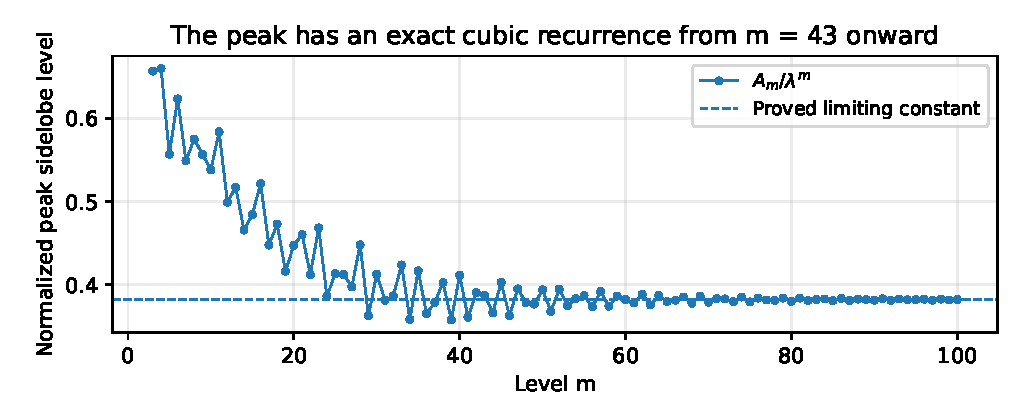
\includegraphics[width=\textwidth]{figures/peak_normalization.pdf}
\caption{The certified normalized peak values and their limiting constant.
The oscillatory transient comes from the two complex roots in
\eqref{eq:binet}; it is not evidence of a failure of the eventual recurrence.}
\end{figure}

\subsection{The shift sequence is also eventually elementary}
The location error is exactly
\begin{equation}
 \frac{k_m^*}{2^m}-\frac23=\frac{(-1)^m}{3\cdot2^m}
 \qquad(m\ge40).
 \label{eq:locationerror}
\end{equation}
Thus the convergence in Tarnu's conjecture has an explicit geometric rate,
and the answer to the nearest-integer question is stronger than infinitude:
every level from $40$ onward works.

Writing $d_m=k_m^*-\ell_m$ for the second column of
Table~\ref{tab:exceptions}, the shift generating function beginning at $m=3$
is
\begin{equation}
 \sum_{m\ge3}k_m^*t^m
 =\frac23\frac{(2t)^3}{1-2t}
  +\frac13\frac{(-t)^3}{1+t}
  +\sum_{m\in\mathcal E}d_mt^m.
 \label{eq:shiftgf}
\end{equation}
In particular, $k_m^*=k_{m-1}^*+2k_{m-2}^*$ for $m\ge42$.
This is another way to express that all the apparent irregularity in the
maximizer locations is confined to a finite initial segment.

\section{Periodic autocorrelations}
\label{sec:periodic}

Define the periodic autocorrelation by
\[
 P_m(k)=\sum_{j=0}^{2^m-1}r_jr_{j+k\bmod2^m}.
\]
Splitting the sum at the wraparound gives
$P_m(k)=C_m(k)+C_m(2^m-k)$ for $0<k<2^m$.
The scalar recurrence immediately yields
\begin{equation}
 P_m(k)=
 \begin{cases}
 4C_{m-2}(|2^{m-1}-k|),&2^{m-2}<k<3\cdot2^{m-2},\ k\ne2^{m-1},\\
 0,&\text{otherwise}.
 \end{cases}
 \label{eq:periodic}
\end{equation}
This reduction is known \citep[Theorem~12]{Tarnu2023}; its derivation also
follows by adding the two branch coordinates in \eqref{eq:branches}.

\begin{corollary}
\label{cor:periodic}
For every $m\ge5$, the periodic absolute maximum is attained at exactly two
positive shifts,
\[
 2^{m-1}-k_{m-2}^*,\qquad 2^{m-1}+k_{m-2}^*,
\]
and its value is $4A_{m-2}$. For every $m\ge42$, these shifts are precisely
\begin{equation}
 \frac{2^m-(-1)^m}{3},\qquad
 \frac{2^{m+1}+(-1)^m}{3},
 \label{eq:periodicmax}
\end{equation}
and the maximum value is $4b_{m-4}$. The threshold $42$ for this pair of
nearest-third locations is sharp.
\end{corollary}
\begin{proof}
For each nonzero argument $t$ with $0<t<2^{m-2}$, exactly two shifts in the
inner half satisfy $|2^{m-1}-k|=t$. Theorem~\ref{thm:main} gives a unique
maximizing argument when $m-2\ge3$. For $m\ge42$, substitute
$k_{m-2}^*=\ell_{m-2}$ and simplify. At $m=41$, the argument comes from the
last exceptional level $39$, so the displayed pair is not maximizing.
\end{proof}

The low levels are separate: $m=3$ gives two periodic maximizing shifts,
whereas $m=4$ gives four, because the underlying aperiodic level $2$ has its
two-way tie. These conventions prevent periodic symmetry from being
mistaken for a failure of the aperiodic uniqueness theorem.

\section{Algorithms, reproducibility, and proof audit}
\label{sec:reproduce}

\subsection{What to run}
From the root of the archive, execute
\begin{lstlisting}
python code/verify.py --output data/verification_summary.json
python code/test_verifier.py
python code/rs_maximum.py 40
\end{lstlisting}
The verifier and the evaluator require only Python's standard library.
Python~3.9 or later is sufficient. The first command rechecks the area draw,
the finite hull certificates, finite word uniqueness, all parametric
containments, the rational projective trap, and direct defining-sum checks
through level $10$. No network access is used.

The separate tests compare every shift with its defining sum through level
$9$, check the polynomial determinant routine against scalar determinants,
exercise acceptance and rejection of tetrahedral witnesses, and compare two
evaluation routes at large levels. They include the last exception $m=39$.

The evaluator accepts an optional \texttt{--shift} argument for an individual
correlation. For the maximum at $m\ge40$, it evaluates $U^{m-2}v$ by repeated
squaring, requiring $O(\log m)$ matrix multiplications. This is an arithmetic
operation count, not a constant-bit-cost claim: the output integers themselves
have size linear in $m$. Evaluating an arbitrary shift uses the address
system and $O(m)$ small-matrix applications.

\subsection{Discovery versus verification}
The discovery scripts use NumPy, SciPy, and SymPy to propose retained
vertices and convenient tetrahedra. Those packages are not part of the
trusted arithmetic path of \texttt{verify.py}. In particular:
\begin{enumerate}[leftmargin=2em,itemsep=0.15em]
\item Numerical hull output supplies only candidate indices. Exact
convex-combination witnesses prove the resulting hull equality.
\item Numerical simplex selection supplies only a triple. Rational
determinants prove containment over the entire parameter rectangle.
\item Approximate eigenvectors motivate a rational center. Exact endpoint
inequalities prove entry and trapping; the proof does not assume that a
rounded vector is an eigenvector.
\end{enumerate}
The certificate-generation scripts and their dependency list are included for
reproducibility. Re-running a hull algorithm can select different valid
triangulations; the certificate verifier checks the mathematical witnesses,
not a particular floating-point triangulation.

\subsection{The executed checks}
The archived execution establishes the following finite obligations:
\begin{center}
\begin{tabular}{lr}
\toprule
Obligation & Verified count or range\\\midrule
Consecutive finite levels & $3\le m\le402$\\
Finite tetrahedral containment witnesses & $11016$\\
Largest retained symmetric generating list & $70$\\
Template generators, including signs & $26$\\
Exact matrix transition identities & $13$\\
Uniform polynomial tetrahedral transitions & $13$\\
Projective return-block length & $6$\\
Defining-sum recurrence comparisons & $2032$\\
Separate unit tests & $6$\\\bottomrule
\end{tabular}
\end{center}
A further exploratory full-array recurrence scan through $m=26$ is supplied
as an independent data file. It agrees with the certified maxima. It is not
used as a substitute for the finite convex-combination certificates.

\subsection{What a subsequent audit should check}
The human-level proof obligations are the scalar recurrence, the address
bijection, the interpretation of the convex-hull certificate, and the
induction connecting the moving polytope to the actual states. They are proved
explicitly in Sections~\ref{sec:recurrence}--\ref{sec:assembly}.
The finite arithmetic obligations are delegated to an executable checker
whose input and acceptance conditions are specified in the article.

Particular attention should be paid to four possible sources of error:
excluding $k=0$ from the peak; separating the two reflected positive shifts;
not confusing a unique vector with a unique word; and distinguishing the
sharp threshold $40$ from the conservative trapping entry $402$.
The proof addresses each of these explicitly.

A successful Python execution does not certify the correctness of the Python
interpreter, nor does it constitute a Lean or another proof-assistant
formalization. The result remains a proposed research proof until its logic
and certificates receive independent scrutiny. Conversely, the argument is
not merely experimental: the finite inequalities establish an induction
covering all larger integers.

\clearpage
\appendix
\section{Randomized area selection and exclusion record}
\label{app:draw}

A fixed list of $100$ mathematical areas was written before choosing the
problem. One $128$-bit seed was drawn from the operating system's random
source, and Python's seeded generator selected an index uniformly using
\texttt{randrange(100)}. The recorded seed is
\begin{center}\ttfamily\small
158962427943756320547759113278578223008
\end{center}
The selected zero-based index was $44$, or \textbf{area $45$: harmonic
analysis}. There were no redraws. The entire list and selection method are
stored in \texttt{data/selection.json}, and the verifier replays the draw.
The source manifest's SHA-256 digest is recorded there as well, binding the
exclusion audit to the supplied version.

\begin{multicols}{3}
\footnotesize
\begin{enumerate}[leftmargin=2.2em,itemsep=0.12em,parsep=0pt]
\item Additive combinatorics
\item Algebraic combinatorics
\item Analytic combinatorics
\item Enumerative combinatorics
\item Extremal set theory
\item Design theory
\item Finite geometry
\item Ramsey theory
\item Graph coloring
\item Structural graph theory
\item Spectral graph theory
\item Graph polynomials
\item Hypergraph theory
\item Matroid theory
\item Combinatorial game theory
\item Discrete geometry
\item Convex geometry
\item Polytope theory
\item Lattice-point enumeration
\item Tiling theory
\item Coding theory
\item Finite fields
\item Finite groups
\item Combinatorial group theory
\item Semigroup theory
\item Ring theory
\item Commutative algebra
\item Polynomial identities
\item Representation theory
\item Invariant theory
\item Linear algebra and matrix inequalities
\item Nonnegative matrices
\item Tensor rank and decomposition
\item Spectral theory
\item Operator inequalities
\item Functional analysis
\item Banach-space geometry
\item Approximation theory
\item Orthogonal polynomials
\item Special functions
\item Real inequalities
\item Complex analysis
\item Univalent functions
\item Potential theory
\item \textbf{Harmonic analysis}
\item Fourier analysis on finite groups
\item Probability inequalities
\item Random walks
\item Markov chains
\item Branching processes
\item Percolation theory
\item Random combinatorial structures
\item Ergodic theory
\item Symbolic dynamics
\item Substitution sequences
\item Automata theory
\item Combinatorics on words
\item Formal languages
\item Type theory
\item Proof theory
\item Computability theory
\item Finite model theory
\item Universal algebra
\item Lattice theory
\item Order theory
\item General topology
\item Topological dynamics
\item Algebraic topology
\item Knot theory
\item Geometric topology
\item Metric geometry
\item Discrete differential geometry
\item Dynamical systems
\item Difference equations
\item Functional equations
\item Iteration theory
\item Asymptotic analysis
\item Diophantine equations
\item Diophantine approximation
\item Arithmetic functions
\item Prime-number theory
\item Modular arithmetic
\item p-adic analysis
\item Transcendental number theory
\item Continued fractions
\item Integer partitions
\item q-series
\item Modular forms
\item Elliptic curves
\item Algebraic number theory
\item Numerical semigroups
\item Combinatorial optimization
\item Integer programming
\item Polyhedral combinatorics
\item Discrete convex analysis
\item Optimization inequalities
\item Information theory
\item Quantum information mathematics
\item Boolean functions
\item Computational geometry

\end{enumerate}
\end{multicols}

\section{Archive map}
The main source is \texttt{article.tex}, with bibliographic metadata in
\texttt{references.bib}, mirrored table data under \texttt{data/}, and two
figures under \texttt{figures/}. The bibliography is embedded in the source;
BibTeX is not required to build the PDF.
\texttt{README.md} gives build and verification commands.
\texttt{STATUS.md} separates the claimed theorem from its review status.
\texttt{notes/proof\_audit.md} records the logical dependencies and the
numerical-to-exact boundary.

The proof-bearing inputs are
\texttt{finite\_certificate.json} and
\texttt{polytope\_certificate.json}. The template matrices are independently
reconstructed by the verifier from the words in \eqref{eq:words}.
The maxima data file is compared with recomputed results, not accepted as an
oracle. The evaluator in \texttt{code/rs\_maximum.py} provides a usable
implementation of the resulting formulas.

\section{Source and scope audit}
\label{sec:sources}

The problem was selected within harmonic analysis after a single randomized
area draw; details are in Appendix~\ref{app:draw}. The supplied
\texttt{manifest(1).tex} was read in full and treated as an exclusion list.
None of its $71$ entries concerns the maximizing shifts of Rudin--Shapiro
aperiodic autocorrelations. Its binary-substitution and determinant topics are
different problems, not alternate versions of this one.

The primary problem source is Tarnu's arXiv version
\texttt{2202.05897v2}, corresponding to the 2023 journal paper. The explicit
later open-status evidence is Conjecture~1.5 in Choi--Tarnu's 2025 paper.
Targeted searches on 20 September 2026 for the conjecture, eventual
maximizers, and a level-$40$ result did not locate a prior resolution of the
statement proved here. This is a bounded literature search, not a guarantee
that no unpublished or unindexed proof exists. The precise sources consulted
and the search terms are recorded in \texttt{notes/sources.md}.

The article does not claim to solve extremal autocorrelation questions for
all binary sequences, arbitrary Golay--Rudin--Shapiro seeds, or general joint
spectral-radius problems. The two matrices, the initial vector, and the
thirteen templates are essential parts of this result.

\begin{thebibliography}{3}
\bibitem[Tarnu(2023)]{Tarnu2023}
Daniel Tarnu.
\newblock On maximal autocorrelations of Rudin--Shapiro sequences.
\newblock \emph{Journal of Approximation Theory} \textbf{287} (2023), 105866.
\newblock \href{https://doi.org/10.1016/j.jat.2023.105866}{doi:10.1016/j.jat.2023.105866}.
\newblock Consulted arXiv version 2, 20 October 2022:
\url{https://arxiv.org/abs/2202.05897v2}.

\bibitem[Choi and Tarnu(2025)]{ChoiTarnu2025}
Stephen Choi and Daniel Tarnu.
\newblock Limiting behavior of Rudin--Shapiro sequence autocorrelations.
\newblock \emph{Transactions of the American Mathematical Society, Series B}
\textbf{12} (2025), 1101--1129.
\newblock \href{https://doi.org/10.1090/btran/237}{doi:10.1090/btran/237}.
\newblock Published 29 August 2025; Conjecture~1.5.
\newblock Author-hosted text:
\url{https://www.sfu.ca/~schoia/paper/rudin-dist.pdf}.

\bibitem[Katz and van der Linden(2022)]{KatzLinden2022}
Daniel J. Katz and Courtney M. van der Linden.
\newblock Peak sidelobe level and peak crosscorrelation of
Golay--Rudin--Shapiro sequences.
\newblock \emph{IEEE Transactions on Information Theory}
\textbf{68}(5) (2022), 3455--3473.
\newblock \href{https://doi.org/10.1109/TIT.2021.3135564}{doi:10.1109/TIT.2021.3135564}.
\newblock \url{https://arxiv.org/abs/2108.07318}.
\end{thebibliography}
\end{document}
